\section{Results}
\subsection{Experiments done in the paper}
Embree considers two examples in his paper, the first one using
\begin{equation}
\mathbf{A} = \begin{pmatrix}
1 & 1 & 1 \\
0 & 1 & 3 \\
0 & 0 & 1 \\
\end{pmatrix}
\;\;\; 
\mathbf{b} = \begin{pmatrix}
2 \\ -4 \\ 1
\end{pmatrix}.
\end{equation}
The second being
\begin{equation}
\mathbf{B} =
\begin{pmatrix}
1 & 2 & -2 \\
0 & 2 & 4 \\
0 & 0 & 3 \\
\end{pmatrix}
\;\;\;
\mathbf{b} =
\begin{pmatrix}
3 \\
1 \\
1 \\
\end{pmatrix}
\end{equation}
Using series expressions as provided in the paper the convergence plots for \texttt{GMRES(1)} and \texttt{GMRES(2)} have been computed, the results shown in figure~\ref{fig:ConvergenceFig1AndFig3} resemble plots one and three in the paper. However to truly understand the gravity of the phenomenon $\mathbf{b}$ has been replaced with 
\begin{equation}
\mathbf{r_0} = \begin{pmatrix}
\xi \\ \eta \\ 1 \\
\end{pmatrix}.
\end{equation}
If $\xi \text{ and } \eta \in [-10,10]$ the plots shown in figures~\ref{fig:fig2} and \ref{fig:fig4}. Can be computed, which are the same as figure 2 and 4, if the different coloring is neglected. These plots show the residual of the two schemes after 30 iterations on a logarithmic scale. Blue areas indicate convergence. 

\begin{figure}
% This file was created by matlab2tikz.
% Minimal pgfplots version: 1.3
%
%The latest updates can be retrieved from
%  http://www.mathworks.com/matlabcentral/fileexchange/22022-matlab2tikz
%where you can also make suggestions and rate matlab2tikz.
%
\documentclass[tikz]{standalone}
\usepackage{pgfplots}
\usepackage{grffile}
\pgfplotsset{compat=newest}
\usetikzlibrary{plotmarks}
\usepackage{amsmath}

\begin{document}
\definecolor{mycolor1}{rgb}{0.00000,0.44700,0.74100}%
\definecolor{mycolor2}{rgb}{0.85000,0.32500,0.09800}%
%
\begin{tikzpicture}

\begin{axis}[%
width=2in,
height=2in,
scale only axis,
xmin=0,
xmax=35,
ymode=log,
ymin=1e-20,
ymax=1,
yminorticks=true,
legend style={legend cell align=left,align=left,draw=white!15!black}
]
\addplot [color=mycolor1,solid,line width=2.0pt]
  table[row sep=crcr]{%
1	1\\
2	0.925820099772552\\
3	0.654653670707977\\
4	2.22044604925031e-16\\
5	2.22044604925031e-16\\
6	2.22044604925031e-16\\
7	2.22044604925031e-16\\
8	2.22044604925031e-16\\
9	2.22044604925031e-16\\
10	2.22044604925031e-16\\
11	2.22044604925031e-16\\
12	2.22044604925031e-16\\
13	2.22044604925031e-16\\
14	2.22044604925031e-16\\
15	2.22044604925031e-16\\
16	2.22044604925031e-16\\
17	2.22044604925031e-16\\
18	2.22044604925031e-16\\
19	2.22044604925031e-16\\
20	2.22044604925031e-16\\
21	2.22044604925031e-16\\
22	2.22044604925031e-16\\
23	2.22044604925031e-16\\
24	2.22044604925031e-16\\
25	2.22044604925031e-16\\
26	2.22044604925031e-16\\
27	2.22044604925031e-16\\
28	2.22044604925031e-16\\
29	2.22044604925031e-16\\
30	2.22044604925031e-16\\
31	2.22044604925031e-16\\
};
\addlegendentry{GMRES(1)};

\addplot [color=mycolor2,solid,line width=2.0pt]
  table[row sep=crcr]{%
1	1\\
2	0.462910049886276\\
3	0.377189160453301\\
4	0.376548629114522\\
5	0.376512989917567\\
6	0.37650248885891\\
7	0.376498558527189\\
8	0.376497022258869\\
9	0.376496407650134\\
10	0.376496158161928\\
11	0.376496055944867\\
12	0.376496013816942\\
13	0.376495996388108\\
14	0.376495989159931\\
15	0.3764959861575\\
16	0.376495984909088\\
17	0.376495984389657\\
18	0.376495984173445\\
19	0.376495984083423\\
20	0.376495984045934\\
21	0.376495984030321\\
22	0.376495984023818\\
23	0.376495984021109\\
24	0.376495984019981\\
25	0.376495984019511\\
26	0.376495984019315\\
27	0.376495984019233\\
28	0.376495984019199\\
29	0.376495984019185\\
30	0.376495984019179\\
31	0.376495984019177\\
};
\addlegendentry{GMRES(2)};

\end{axis}
\end{tikzpicture}%
\end{document}
% This file was created by matlab2tikz.
% Minimal pgfplots version: 1.3
%
%The latest updates can be retrieved from
%  http://www.mathworks.com/matlabcentral/fileexchange/22022-matlab2tikz
%where you can also make suggestions and rate matlab2tikz.
%
\documentclass[tikz]{standalone}
\usepackage{pgfplots}
\usepackage{grffile}
\pgfplotsset{compat=newest}
\usetikzlibrary{plotmarks}
\usepackage{amsmath}

\begin{document}
\definecolor{mycolor1}{rgb}{0.00000,0.44700,0.74100}%
\definecolor{mycolor2}{rgb}{0.85000,0.32500,0.09800}%
%
\begin{tikzpicture}

\begin{axis}[%
width=2in,
height=2in,
scale only axis,
xmin=0,
xmax=35,
ymode=log,
ymin=1e-20,
ymax=1,
yminorticks=true,
legend style={legend cell align=left,align=left,draw=white!15!black}
]
\addplot [color=mycolor1,solid,line width=2.0pt]
  table[row sep=crcr]{%
1	1\\
2	0.674199862463242\\
3	0.603022689155527\\
4	2.22044604925031e-16\\
5	2.22044604925031e-16\\
6	2.22044604925031e-16\\
7	2.22044604925031e-16\\
8	2.22044604925031e-16\\
9	2.22044604925031e-16\\
10	2.22044604925031e-16\\
11	2.22044604925031e-16\\
12	2.22044604925031e-16\\
13	2.22044604925031e-16\\
14	2.22044604925031e-16\\
15	2.22044604925031e-16\\
16	2.22044604925031e-16\\
17	2.22044604925031e-16\\
18	2.22044604925031e-16\\
19	2.22044604925031e-16\\
20	2.22044604925031e-16\\
21	2.22044604925031e-16\\
22	2.22044604925031e-16\\
23	2.22044604925031e-16\\
24	2.22044604925031e-16\\
25	2.22044604925031e-16\\
26	2.22044604925031e-16\\
27	2.22044604925031e-16\\
28	2.22044604925031e-16\\
29	2.22044604925031e-16\\
30	2.22044604925031e-16\\
31	2.22044604925031e-16\\
};
\addlegendentry{GMRES(1)};

\addplot [color=mycolor2,solid,line width=2.0pt]
  table[row sep=crcr]{%
1	1\\
2	0.426401432711221\\
3	0.147341893736751\\
4	0.14430093184878\\
5	0.144075571440941\\
6	0.144047064375947\\
7	0.144042732325566\\
8	0.144042026003053\\
9	0.144041907542309\\
10	0.144041887444274\\
11	0.144041884018229\\
12	0.144041883433058\\
13	0.14404188333303\\
14	0.144041883315925\\
15	0.144041883313\\
16	0.1440418833125\\
17	0.144041883312414\\
18	0.144041883312399\\
19	0.144041883312397\\
20	0.144041883312396\\
21	0.144041883312396\\
22	0.144041883312396\\
23	0.144041883312396\\
24	0.144041883312396\\
25	0.144041883312396\\
26	0.144041883312396\\
27	0.144041883312396\\
28	0.144041883312396\\
29	0.144041883312396\\
30	0.144041883312396\\
31	0.144041883312396\\
};
\addlegendentry{GMRES(2)};

\end{axis}
\end{tikzpicture}%
\end{document}
\caption{Convergence plot of GMRES(1) and GMRES(2). For matrix $\mathbf{A}$ (left), as seen in figure 1 of Embree's paper and for matrix $\mathbf{B}$ (right), as shown in figure three of Embree's paper.}
\label{fig:ConvergenceFig1AndFig3}
\end{figure}

\begin{figure}
\centering
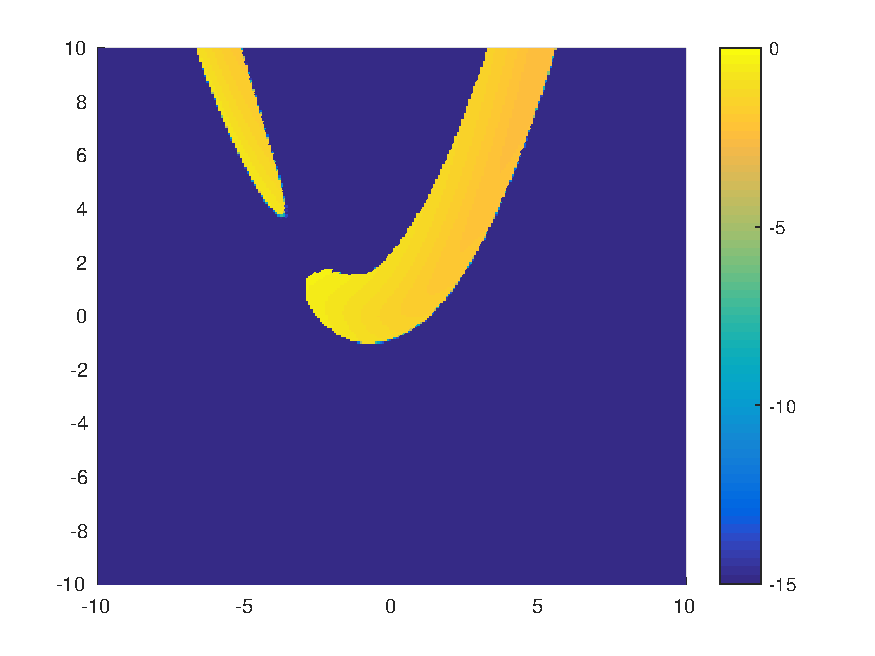
\includegraphics[width=0.45\linewidth]{../src/figure/fig2Matp1}
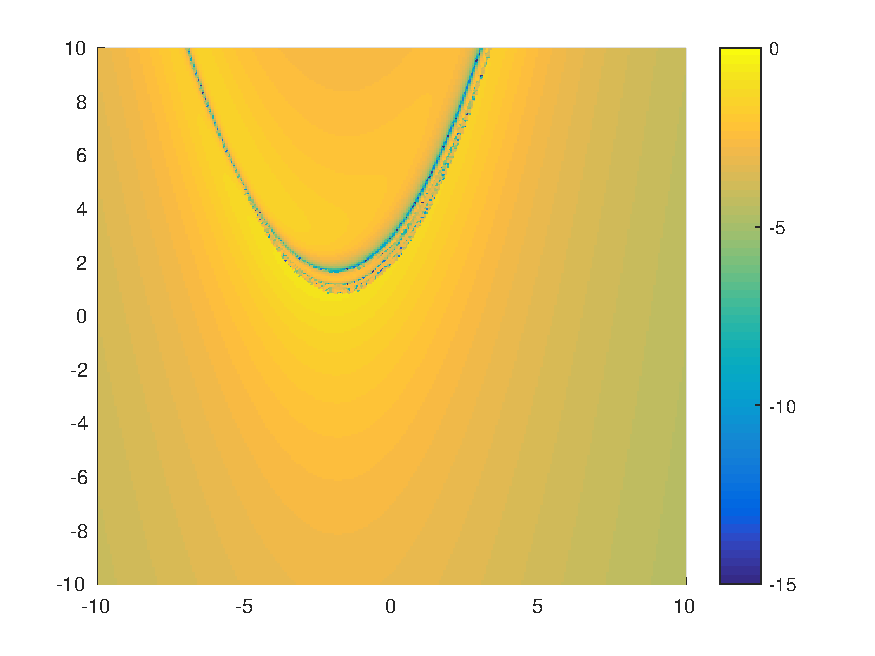
\includegraphics[width=0.45\linewidth]{../src/figure/fig2Matp2}
\caption{Residual magnitude Plot for matrix $\mathbf{A}$, as seen in the Embree paper GMRES(1)(left) and GMRES(2)(right) in figure two.}
\label{fig:fig2}
\end{figure}

\begin{figure}
\centering
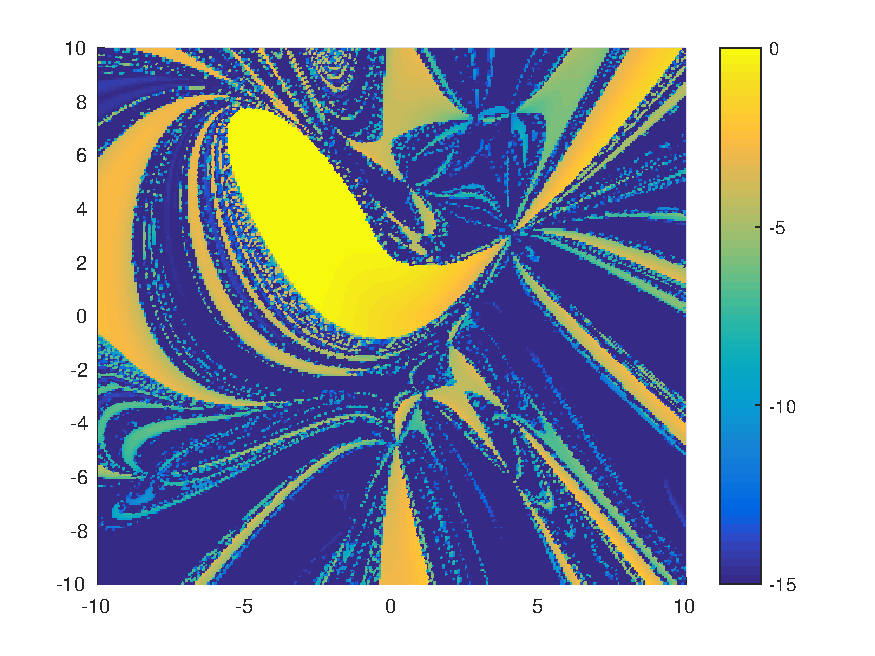
\includegraphics[width=0.45\linewidth]{../src/figure/fig4Matp2}
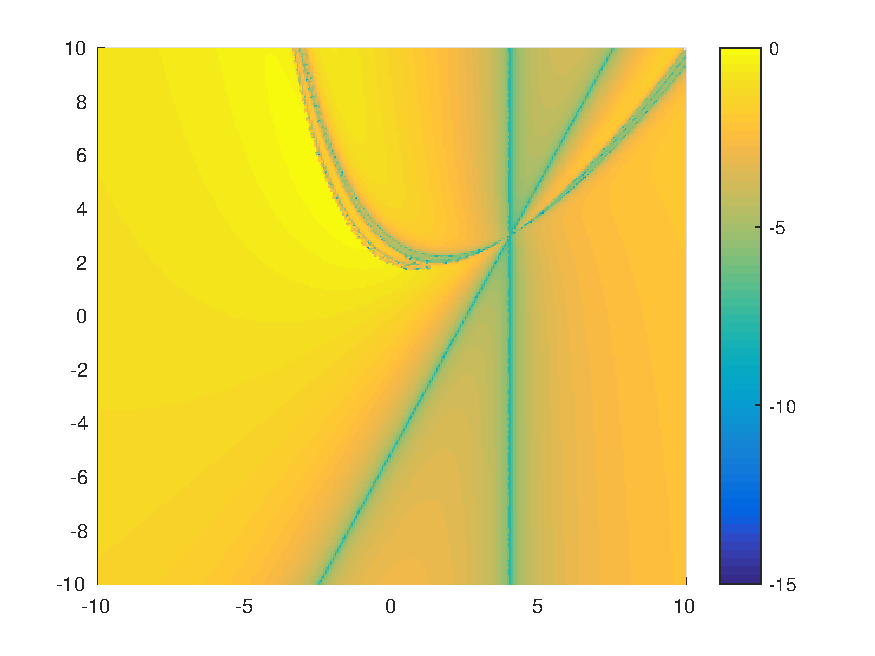
\includegraphics[width=0.45\linewidth]{../src/figure/fig4Matp1}
\caption{Residual magnitude Plot for matrix $\mathbf{B}$, as seen in the Embree paper for GMRES(1)(left) and GMRES(2)(right) in figure 4.}
\label{fig:fig4}
\end{figure}

\subsection{Additional experiments}
If $A - 0.35*\mathbf{I}$ is considered the condition number changes from $\kappa(\mathbf{A}) = 14.2950$ to  $\kappa(\mathbf{A} - 0.35*\mathbf{I}) = 39.1873$. At the same time the convergent area of \texttt{GMRES(1)} shown in figure~\ref{fig:modA}, shrinks considerably in comparison to the plot~\ref{fig:fig2}. Additionally as the conditioning worsened the white foggy areas without convergence grew significantly. 
\begin{figure}
\centering
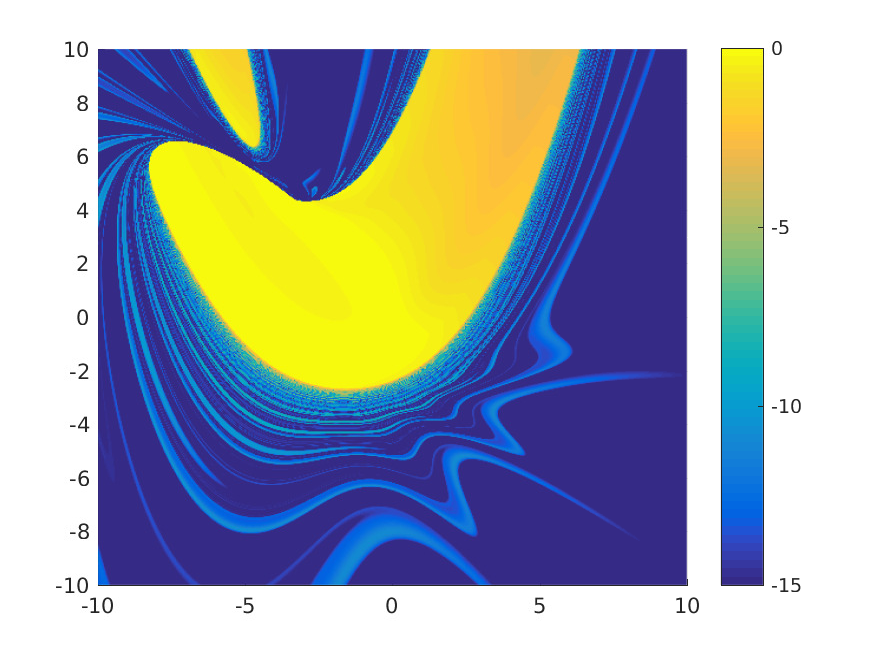
\includegraphics[width=0.45\linewidth]{../src/figure/Am0p35eyeGMRES1}
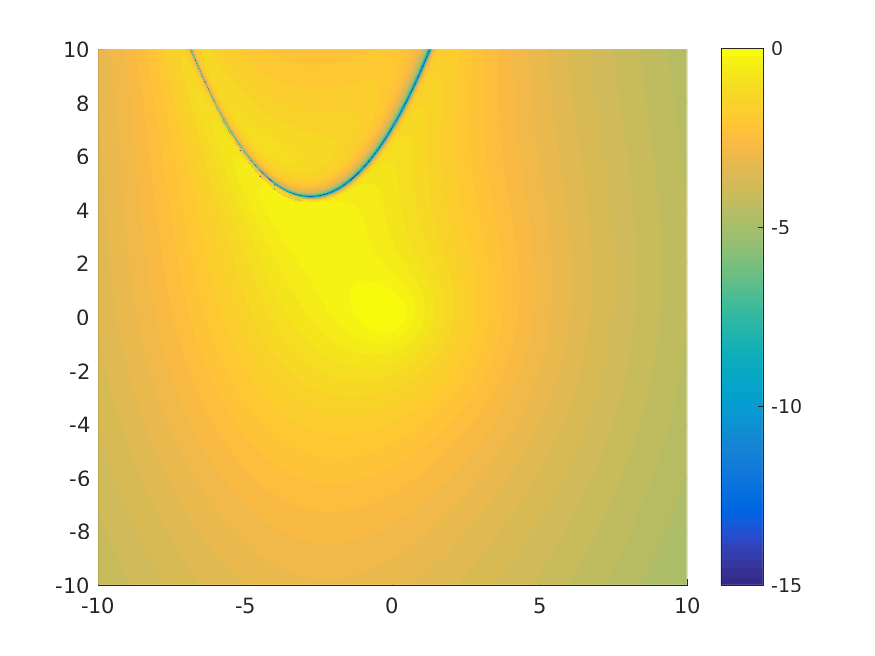
\includegraphics[width=0.45\linewidth]{../src/figure/Am0p35eyeGMRES2}
\caption{\texttt{GMRES(1)} and \texttt{GMRES(2)} convergence on $\mathbf{A} - 0.35 \cdot \mathbf{I}$.  } 
\label{fig:modA}
\end{figure}

In a second series of experiments, designed to further investigate the effect of changed conditioning, $\mathbf{A}$ will be filled with entries drawn from the standart normal distribution ($\mu = 0$, $\sigma^2 = 1$). The values turned out to be:
\begin{equation}
\mathbf{R} = \begin{pmatrix}
-0.3034 &   0.8884 &  -0.8095 \\
 0.2939 &  -1.1471 &  -2.9443 \\
-0.7873 &  -1.0689 &   1.4384 \\
\end{pmatrix} 
\end{equation}
Results for \texttt{GMRES(1)} and \texttt{GMRES(2)}. Are shown in figure \ref{fig:randAGMRES2}. Here it can be observed, that \texttt{GMRES(2)}, converges for all possible right hand sides $\mathbf{b}$, while \texttt{GMRES(1)} does not. This is probably the more common, but mathematically less interesting case. Often convergence improves significantly if the identity matrix is added to A. Unfortunately the condition number got worse by adding one multiple of the identity. It increased from $\kappa(\mathbf{R})=5.1025$ to $\kappa(\mathbf{R} + \mathbf{I})=32.4770$. Adding two dimes the identity matrix makes matters even worse as $\kappa(\mathbf{R} + 2\mathbf{I})=77.5446$, with results shown in figure~\ref{fig:randAp2eyeGMRES2}. Finally adding three times the identity leads to $\kappa(\mathbf{R} + 3\mathbf{I})=6.4262$ and complete convergence for both algorithms figure~\ref{fig:randAp3eyeGMRES2}. However the conditioning is still worse then it was originally, which indicates that conditioning alone can not be used to predict \texttt{GMRES(m)} convergence. 

\begin{figure}
\centering
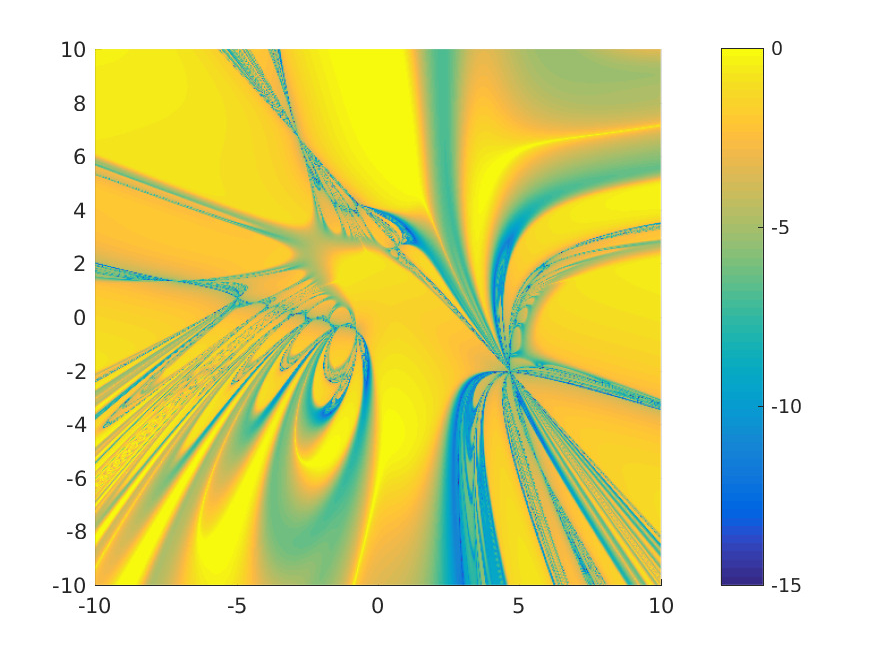
\includegraphics[width=0.45\linewidth]{../src/figure/randAGMRES1}
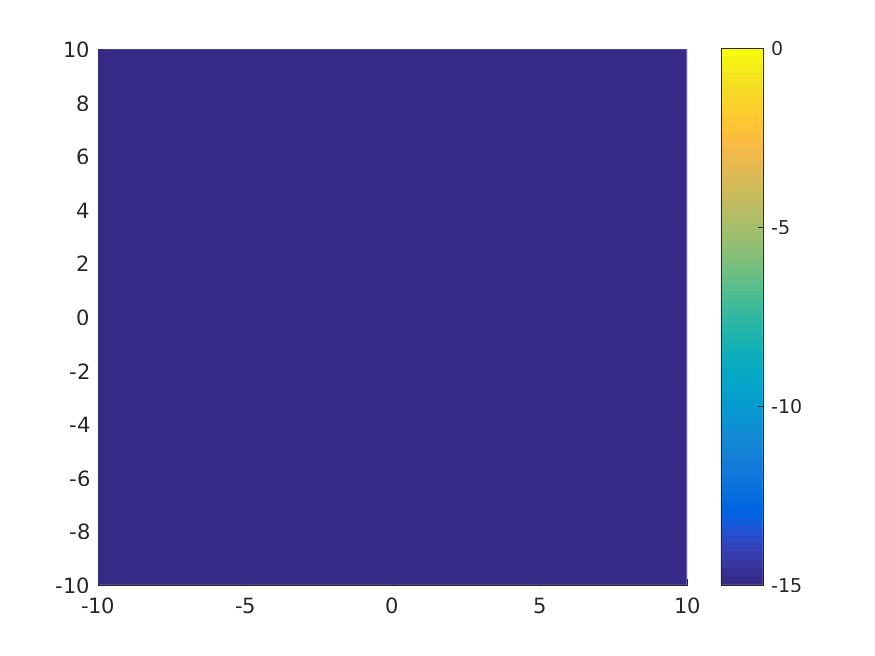
\includegraphics[width=0.45\linewidth]{../src/figure/randAGMRES2}
\caption{Convergence of \texttt{GMRES(1)}(left) and \texttt{GMRES(2)}(right) for the random matrix $\mathbf{R}$.}
\label{fig:randAGMRES2}
\end{figure}
\begin{figure}
\centering
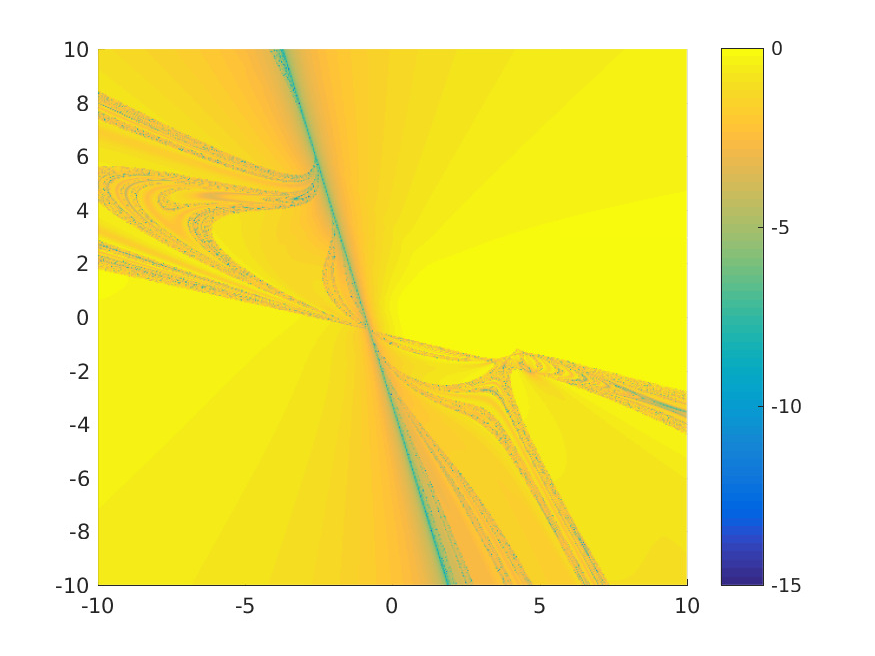
\includegraphics[width=0.45\linewidth]{../src/figure/randAp2eyeGMRES1}
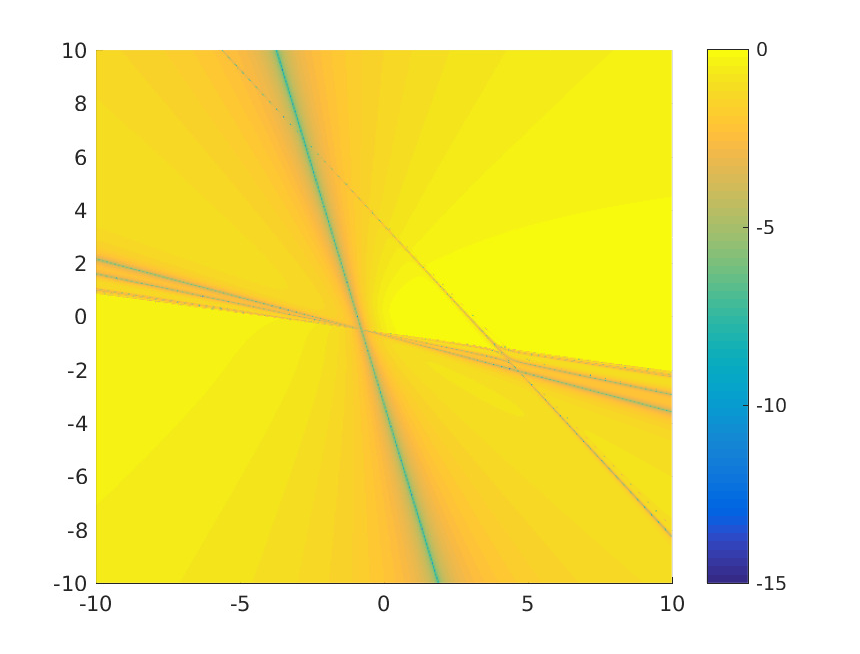
\includegraphics[width=0.45\linewidth]{../src/figure/randAp2eyeGMRES2}
\caption{Convergence results for $\mathbf{R} + 2\mathbf{I}$}
\label{fig:randAp2eyeGMRES2}
\end{figure}
\begin{figure}
\centering
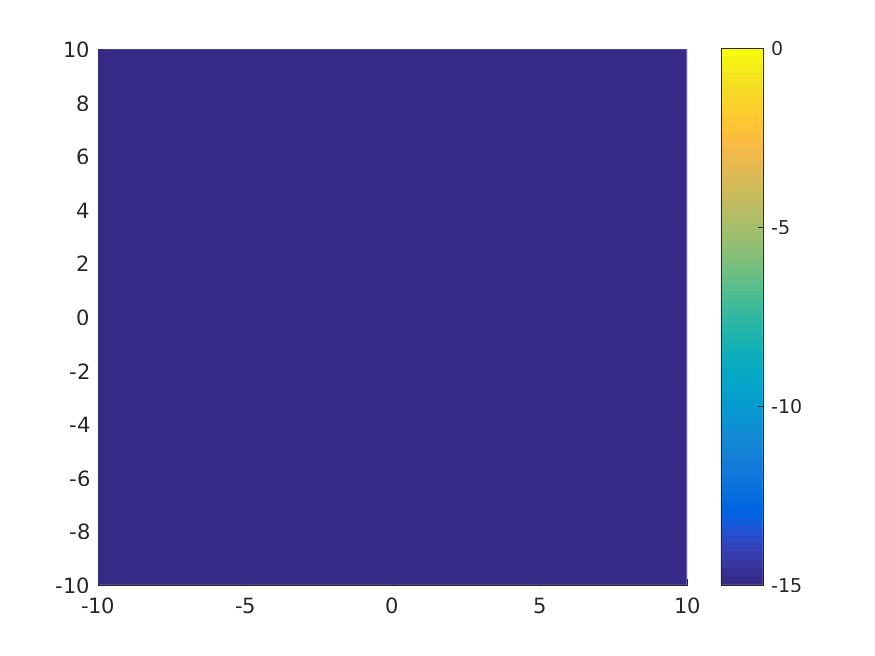
\includegraphics[width=0.45\linewidth]{../src/figure/randAp3eyeGMRES2}
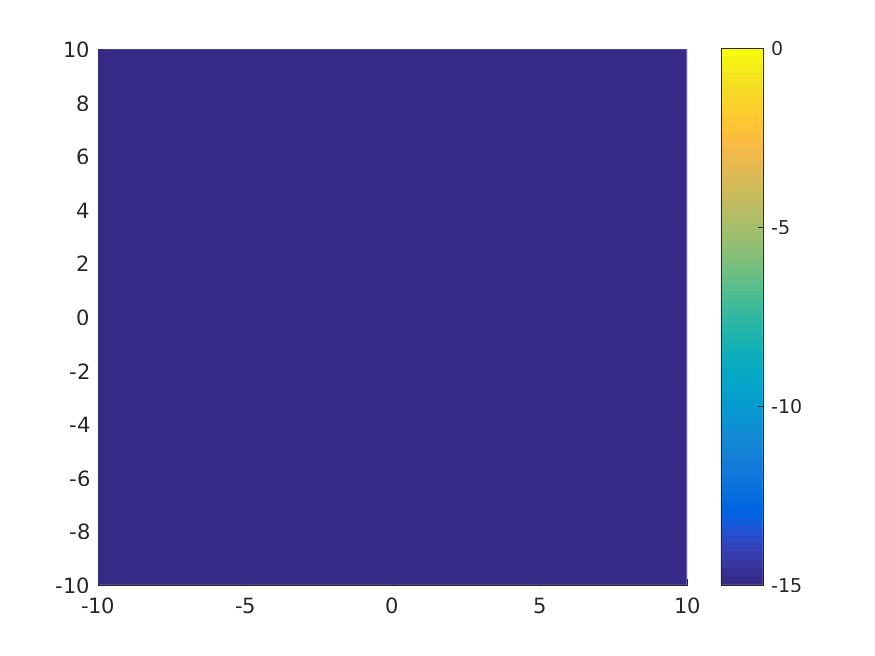
\includegraphics[width=0.45\linewidth]{../src/figure/randAp3eyeGMRES2}
\caption{Convergence results for $\mathbf{R} + 3\mathbf{I}$}
\label{fig:randAp3eyeGMRES2}
\end{figure}

\subsection{Two-Dimensional case}
At the end of the paper Embree proposes to take a closer look at:
\begin{equation}
\mathbf{C} = \begin{pmatrix}
1 & -2 \\
0 & 1 \\
\end{pmatrix}
\;\;\;
\mathbf{r_0} = \begin{pmatrix} \xi \\ \eta \end{pmatrix}
\end{equation}
The residuals show noisy convergence patterns in the bottom and top corners for \texttt{GMRES(1)} in figure~\ref{fig:fig4}. On the right side seemingly random patterns are shown at larger magnification.
Similar ones appeared in figure \ref{fig:fig4} when zooming in. No plot exists for \texttt{GMRES(2)} is it always converged completely within two iterations. In fact for all of the approximately ten two by two matrices that where tried did \texttt{GMRES(2)} converge to the exact result.

\begin{figure}
\centering
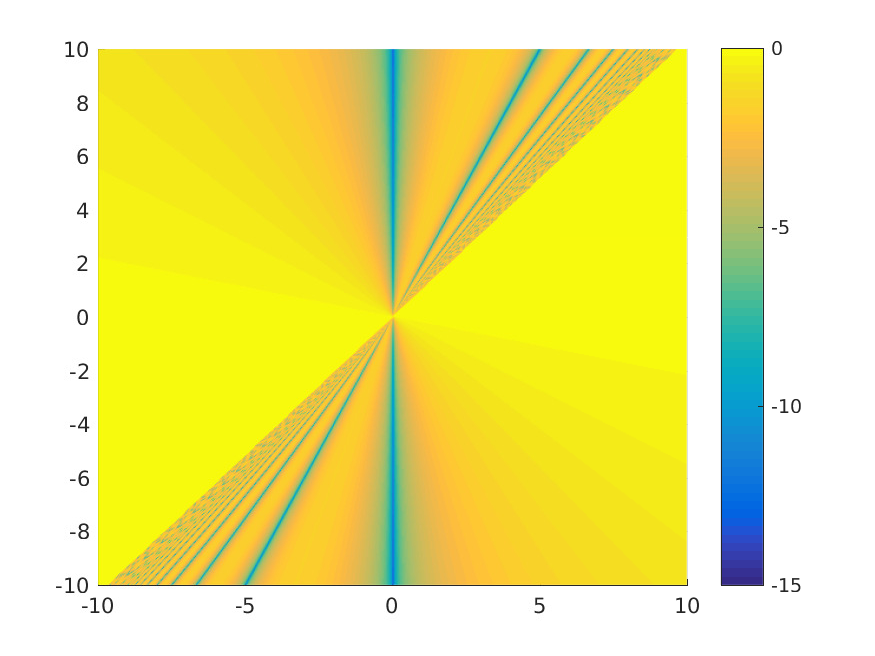
\includegraphics[width=0.45\linewidth]{../src/figure/twoDPaper}
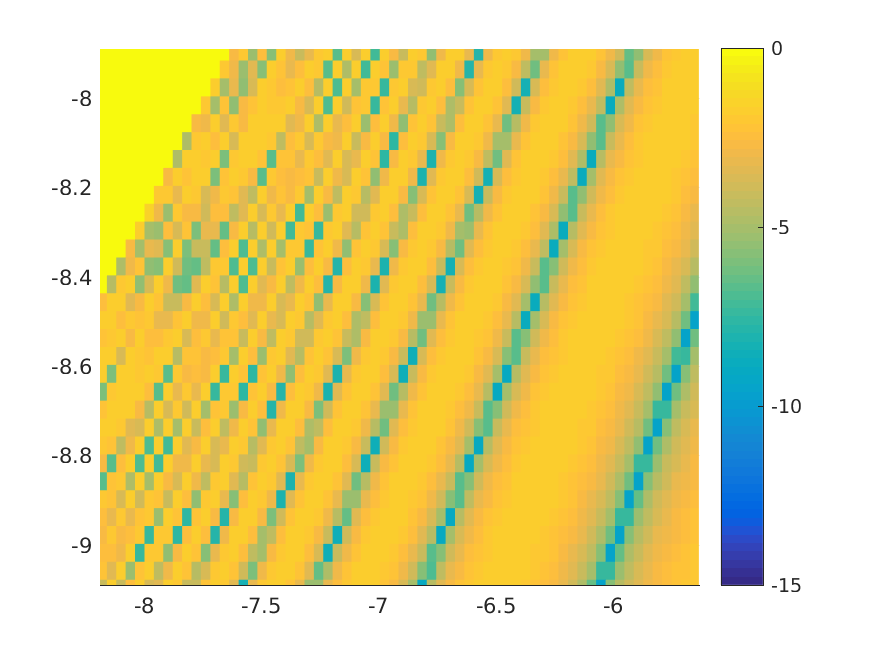
\includegraphics[width=0.45\linewidth]{../src/figure/twoDZoom}
\caption{A plot of the convergence plain for the matrix $\mathbf{C}$ proposed at the end of Embree's paper. With zoom on an interesting region.}
\label{fig:twoDZoom}
\end{figure}




